\usetikzlibrary{calc}
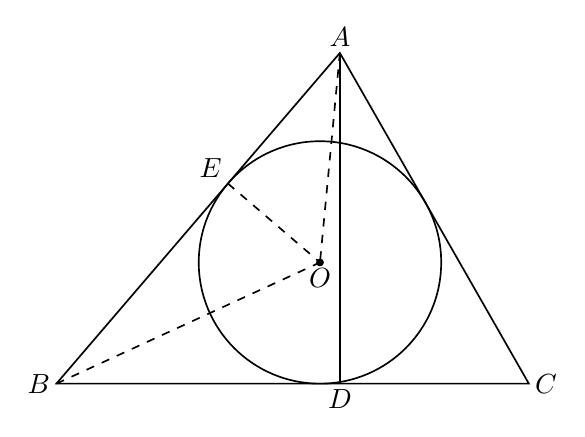
\begin{tikzpicture}[x=1cm,y=1cm,line width=.6pt,font=\normalsize]
\coordinate (A) at (0.6,4.2);
\coordinate (B) at (-3,0);
\coordinate (C) at (3,0);
\coordinate (D) at (0.6,0);
\coordinate (O) at (0.3472,1.5395);
\coordinate (E) at (-0.8217,2.5414);
\draw[solid] (A)--(B)--(C)--cycle;
\draw[solid] (A)--(D);
\draw[dashed] (A)--(O);
\draw[dashed] (B)--(O);
\draw[dashed] (E)--(O);
\draw[solid] (O) circle[radius=1.5395cm];
\fill (O) circle[radius=.045cm];
\node[above=2pt,inner sep=0pt] at (A) {$A$};
\node[left=2pt,inner sep=0pt] at (B) {$B$};
\node[right=2pt,inner sep=0pt] at (C) {$C$};
\node[below=2pt,inner sep=0pt] at (D) {$D$};
\node[above left=2pt,inner sep=0pt] at (E) {$E$};
\node[below=2pt,inner sep=0pt] at (O) {$O$};

% Explicit named circle-center points, painted after all region fills.
\fill (O) circle[radius=1.4pt];
\end{tikzpicture}
